% Options for packages loaded elsewhere
\PassOptionsToPackage{unicode}{hyperref}
\PassOptionsToPackage{hyphens}{url}
%
\documentclass[
  man]{apa6}
\usepackage{amsmath,amssymb}
\usepackage{iftex}
\ifPDFTeX
  \usepackage[T1]{fontenc}
  \usepackage[utf8]{inputenc}
  \usepackage{textcomp} % provide euro and other symbols
\else % if luatex or xetex
  \usepackage{unicode-math} % this also loads fontspec
  \defaultfontfeatures{Scale=MatchLowercase}
  \defaultfontfeatures[\rmfamily]{Ligatures=TeX,Scale=1}
\fi
\usepackage{lmodern}
\ifPDFTeX\else
  % xetex/luatex font selection
\fi
% Use upquote if available, for straight quotes in verbatim environments
\IfFileExists{upquote.sty}{\usepackage{upquote}}{}
\IfFileExists{microtype.sty}{% use microtype if available
  \usepackage[]{microtype}
  \UseMicrotypeSet[protrusion]{basicmath} % disable protrusion for tt fonts
}{}
\makeatletter
\@ifundefined{KOMAClassName}{% if non-KOMA class
  \IfFileExists{parskip.sty}{%
    \usepackage{parskip}
  }{% else
    \setlength{\parindent}{0pt}
    \setlength{\parskip}{6pt plus 2pt minus 1pt}}
}{% if KOMA class
  \KOMAoptions{parskip=half}}
\makeatother
\usepackage{xcolor}
\usepackage{graphicx}
\makeatletter
\def\maxwidth{\ifdim\Gin@nat@width>\linewidth\linewidth\else\Gin@nat@width\fi}
\def\maxheight{\ifdim\Gin@nat@height>\textheight\textheight\else\Gin@nat@height\fi}
\makeatother
% Scale images if necessary, so that they will not overflow the page
% margins by default, and it is still possible to overwrite the defaults
% using explicit options in \includegraphics[width, height, ...]{}
\setkeys{Gin}{width=\maxwidth,height=\maxheight,keepaspectratio}
% Set default figure placement to htbp
\makeatletter
\def\fps@figure{htbp}
\makeatother
\setlength{\emergencystretch}{3em} % prevent overfull lines
\providecommand{\tightlist}{%
  \setlength{\itemsep}{0pt}\setlength{\parskip}{0pt}}
\setcounter{secnumdepth}{-\maxdimen} % remove section numbering
% Make \paragraph and \subparagraph free-standing
\makeatletter
\ifx\paragraph\undefined\else
  \let\oldparagraph\paragraph
  \renewcommand{\paragraph}{
    \@ifstar
      \xxxParagraphStar
      \xxxParagraphNoStar
  }
  \newcommand{\xxxParagraphStar}[1]{\oldparagraph*{#1}\mbox{}}
  \newcommand{\xxxParagraphNoStar}[1]{\oldparagraph{#1}\mbox{}}
\fi
\ifx\subparagraph\undefined\else
  \let\oldsubparagraph\subparagraph
  \renewcommand{\subparagraph}{
    \@ifstar
      \xxxSubParagraphStar
      \xxxSubParagraphNoStar
  }
  \newcommand{\xxxSubParagraphStar}[1]{\oldsubparagraph*{#1}\mbox{}}
  \newcommand{\xxxSubParagraphNoStar}[1]{\oldsubparagraph{#1}\mbox{}}
\fi
\makeatother
% definitions for citeproc citations
\NewDocumentCommand\citeproctext{}{}
\NewDocumentCommand\citeproc{mm}{%
  \begingroup\def\citeproctext{#2}\cite{#1}\endgroup}
\makeatletter
 % allow citations to break across lines
 \let\@cite@ofmt\@firstofone
 % avoid brackets around text for \cite:
 \def\@biblabel#1{}
 \def\@cite#1#2{{#1\if@tempswa , #2\fi}}
\makeatother
\newlength{\cslhangindent}
\setlength{\cslhangindent}{1.5em}
\newlength{\csllabelwidth}
\setlength{\csllabelwidth}{3em}
\newenvironment{CSLReferences}[2] % #1 hanging-indent, #2 entry-spacing
 {\begin{list}{}{%
  \setlength{\itemindent}{0pt}
  \setlength{\leftmargin}{0pt}
  \setlength{\parsep}{0pt}
  % turn on hanging indent if param 1 is 1
  \ifodd #1
   \setlength{\leftmargin}{\cslhangindent}
   \setlength{\itemindent}{-1\cslhangindent}
  \fi
  % set entry spacing
  \setlength{\itemsep}{#2\baselineskip}}}
 {\end{list}}
\usepackage{calc}
\newcommand{\CSLBlock}[1]{\hfill\break\parbox[t]{\linewidth}{\strut\ignorespaces#1\strut}}
\newcommand{\CSLLeftMargin}[1]{\parbox[t]{\csllabelwidth}{\strut#1\strut}}
\newcommand{\CSLRightInline}[1]{\parbox[t]{\linewidth - \csllabelwidth}{\strut#1\strut}}
\newcommand{\CSLIndent}[1]{\hspace{\cslhangindent}#1}
\ifLuaTeX
\usepackage[bidi=basic]{babel}
\else
\usepackage[bidi=default]{babel}
\fi
\babelprovide[main,import]{english}
% get rid of language-specific shorthands (see #6817):
\let\LanguageShortHands\languageshorthands
\def\languageshorthands#1{}
% Manuscript styling
\usepackage{upgreek}
\captionsetup{font=singlespacing,justification=justified}

% Table formatting
\usepackage{longtable}
\usepackage{lscape}
% \usepackage[counterclockwise]{rotating}   % Landscape page setup for large tables
\usepackage{multirow}		% Table styling
\usepackage{tabularx}		% Control Column width
\usepackage[flushleft]{threeparttable}	% Allows for three part tables with a specified notes section
\usepackage{threeparttablex}            % Lets threeparttable work with longtable

% Create new environments so endfloat can handle them
% \newenvironment{ltable}
%   {\begin{landscape}\centering\begin{threeparttable}}
%   {\end{threeparttable}\end{landscape}}
\newenvironment{lltable}{\begin{landscape}\centering\begin{ThreePartTable}}{\end{ThreePartTable}\end{landscape}}

% Enables adjusting longtable caption width to table width
% Solution found at http://golatex.de/longtable-mit-caption-so-breit-wie-die-tabelle-t15767.html
\makeatletter
\newcommand\LastLTentrywidth{1em}
\newlength\longtablewidth
\setlength{\longtablewidth}{1in}
\newcommand{\getlongtablewidth}{\begingroup \ifcsname LT@\roman{LT@tables}\endcsname \global\longtablewidth=0pt \renewcommand{\LT@entry}[2]{\global\advance\longtablewidth by ##2\relax\gdef\LastLTentrywidth{##2}}\@nameuse{LT@\roman{LT@tables}} \fi \endgroup}

% \setlength{\parindent}{0.5in}
% \setlength{\parskip}{0pt plus 0pt minus 0pt}

% Overwrite redefinition of paragraph and subparagraph by the default LaTeX template
% See https://github.com/crsh/papaja/issues/292
\makeatletter
\renewcommand{\paragraph}{\@startsection{paragraph}{4}{\parindent}%
  {0\baselineskip \@plus 0.2ex \@minus 0.2ex}%
  {-1em}%
  {\normalfont\normalsize\bfseries\itshape\typesectitle}}

\renewcommand{\subparagraph}[1]{\@startsection{subparagraph}{5}{1em}%
  {0\baselineskip \@plus 0.2ex \@minus 0.2ex}%
  {-\z@\relax}%
  {\normalfont\normalsize\itshape\hspace{\parindent}{#1}\textit{\addperi}}{\relax}}
\makeatother

\makeatletter
\usepackage{etoolbox}
\patchcmd{\maketitle}
  {\section{\normalfont\normalsize\abstractname}}
  {\section*{\normalfont\normalsize\abstractname}}
  {}{\typeout{Failed to patch abstract.}}
\patchcmd{\maketitle}
  {\section{\protect\normalfont{\@title}}}
  {\section*{\protect\normalfont{\@title}}}
  {}{\typeout{Failed to patch title.}}
\makeatother

\usepackage{xpatch}
\makeatletter
\xapptocmd\appendix
  {\xapptocmd\section
    {\addcontentsline{toc}{section}{\appendixname\ifoneappendix\else~\theappendix\fi\\: #1}}
    {}{\InnerPatchFailed}%
  }
{}{\PatchFailed}
\DeclareDelayedFloatFlavor{ThreePartTable}{table}
\DeclareDelayedFloatFlavor{lltable}{table}
\DeclareDelayedFloatFlavor*{longtable}{table}
\makeatletter
\renewcommand{\efloat@iwrite}[1]{\immediate\expandafter\protected@write\csname efloat@post#1\endcsname{}}
\makeatother
\usepackage{lineno}

\linenumbers
\usepackage{csquotes}
\ifLuaTeX
  \usepackage{selnolig}  % disable illegal ligatures
\fi
\usepackage{bookmark}
\IfFileExists{xurl.sty}{\usepackage{xurl}}{} % add URL line breaks if available
\urlstyle{same}
\hypersetup{
  pdftitle={Understanding Housing Market Trends and Risks : An Analytical Study},
  pdfauthor={Kunal Bhardwaj1},
  pdflang={en-EN},
  hidelinks,
  pdfcreator={LaTeX via pandoc}}

\title{Understanding Housing Market Trends and Risks : An Analytical Study}
\author{Kunal Bhardwaj\textsuperscript{1}}
\date{}


\shorttitle{Housing Market Trends and Risks}

\authornote{

STAT 429: Time Series Analysis

The authors made the following contributions. Kunal Bhardwaj: Conceptualization, Data Curation, Visualization, Writing - Original Draft Preparation, Writing - Review \& Editing.

}

\affiliation{\vspace{0.5cm}\textsuperscript{1} UIUC}

\abstract{%
The objective of this study is to arrive at a model to predict the median sales price of houses sold in the US. The study tries to find the most significant predictors of price based on a regression analysis. A further ARCH-based analysis will try to estimate the volatility in house prices.
The study finds that `Median Sales Price of Houses Sold' and `30 Year Fixed Rate Mortgage Average' are significant predictors of housing prices. The forecasting performance for ARIMA and ARCH models were found to be fairly similar.

The study found that homeownership rate is not a significant predictor of median housing prices. It was also found that ARCH models failed to capture volatility patterns with a high degree of satisfaction. This may be due to the fact that the US housing market has been historically been very stable and immune to price shocks in the past.
The results from all the selected models reveal that median house prices will remain stable or will go down slightly over the next five quarters.
}



\begin{document}
\maketitle

\section{Introduction}\label{introduction}

\emph{Federal Reserve Economic Data (FRED)} is a comprehensive database maintained by the Federal Reserve Bank of St.~Louis. It provides access to a wide range of economic data, including economic indicators, financial and banking data, monetary data, and regional data for the United States. FRED aggregates data from various government agencies, international organizations, and other sources, making it a valuable resource for researchers, economists, policymakers, and the general public.

The dataset retrieved from \emph{FRED} website comprises of six time series:

\begin{enumerate}
\def\labelenumi{\roman{enumi})}
\item
  Median Sales Price of Houses Sold for the United States
\item
  Monthly supply of New Houses in the United States
\item
  New Privately owned Housing units started
\item
  Home ownership rate in the United States
\item
  30 Year Fixed Rate Mortgage Average in the United States
\item
  Consumer Price Index (CPI) for All Urban Consumers: All Items Less Shelter in U.S. City Average
\end{enumerate}

The objective of the project will be to predict Median Price \emph{(i)} based on four other factors \emph{(ii), (iii), (iv) \& (v)}. The CPI data \emph{(vi)} will not be used as a predictor but will be used to adjust Median Price based on inflation.

These four variables are fundamental drivers influencing the supply and demand dynamics of the housing market. For instance, the monthly supply of new houses and new housing units started \emph{(ii)} offer insights into the supply side of the market, while the home ownership rate \emph{(iv)} reflects the demand for housing. Moreover, the 30 year fixed rate mortgage average \emph{(v)} directly impacts affordability and purchasing power, crucial factors influencing housing demand. The structure of the data is outlined below.

\subsection{\texorpdfstring{Median Sales Price of Houses Sold for the United States (MSPUS) {[}Quarterly{]} {[}Q1'63 Q4'23{]} \emph{OUTCOME VARIABLE}}{Median Sales Price of Houses Sold for the United States (MSPUS) {[}Quarterly{]} {[}Q1'63 Q4'23{]} OUTCOME VARIABLE}}\label{median-sales-price-of-houses-sold-for-the-united-states-mspus-quarterly-q163-q423-outcome-variable}

The Median Sales Price of Houses Sold for the United States in US Dollars. The original data has not been seasonally adjusted.

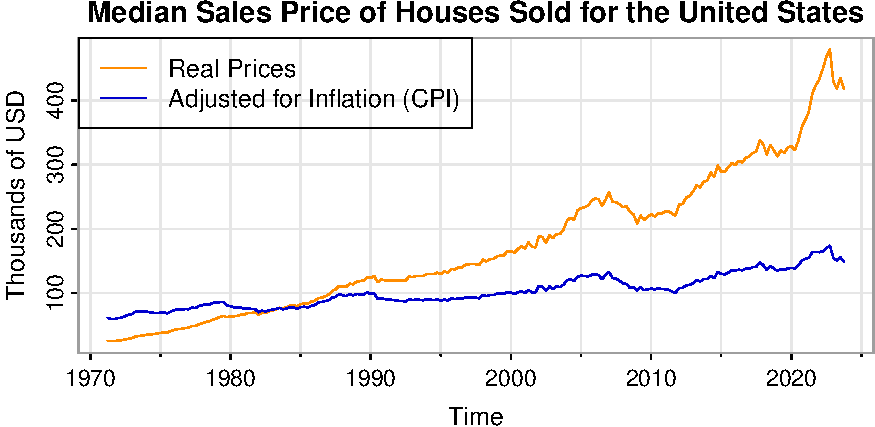
\includegraphics{STAT429Report---Copy_files/figure-latex/unnamed-chunk-2-1.pdf}
From the plot of Median Sales Price of Houses Sold, we can see that there exists an obvious trend in the data. The Median Prices will be adjusted for inflation based on 1982:1984 prices to make median housing prices from different years directly comparable. This is crucial for understanding long term trends in housing prices and assessing changes in affordability over time.

Moreover, adjusting median housing prices for inflation should lead to more accurate forecasts by avoid biases introduced by price shocks in commodity prices, the effect of which have not been included in the model.

\subsection{\texorpdfstring{Monthly Supply of New Houses in the United States (MSACSR) {[}Monthly{]} {[}Jan'63 - Dec'23{]} \emph{Predictor variable 1}}{Monthly Supply of New Houses in the United States (MSACSR) {[}Monthly{]} {[}Jan'63 - Dec'23{]} Predictor variable 1}}\label{monthly-supply-of-new-houses-in-the-united-states-msacsr-monthly-jan63---dec23-predictor-variable-1}

The months' supply is the ratio of new houses for sale to new houses sold. This statistic provides an indication of the size of the new for-sale inventory in relation to the number of new houses currently being sold. The months' supply indicates how long the current new for-sale inventory would last given the current sales rate if no additional new houses were built.
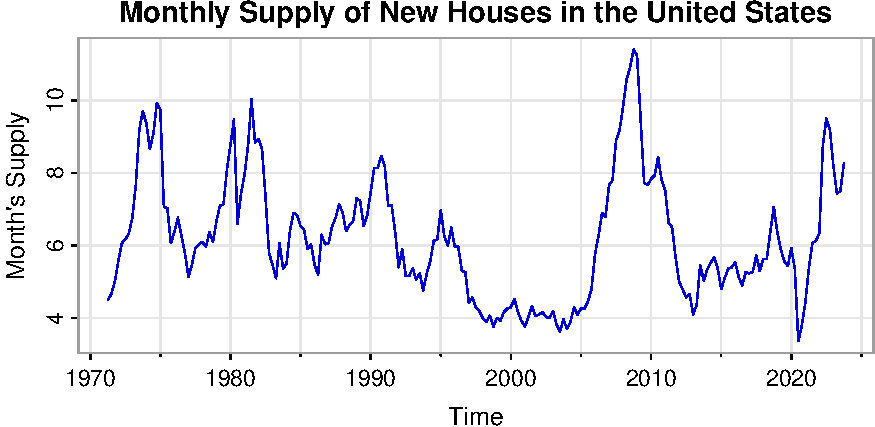
\includegraphics{STAT429Report---Copy_files/figure-latex/unnamed-chunk-3-1.pdf}

\subsection{\texorpdfstring{New Privately-Owned Housing Units Started: Total Units (HOUST) {[}Monthly{]} {[}Jan'59 - Jan'24{]} \emph{Predictor variable 2}}{New Privately-Owned Housing Units Started: Total Units (HOUST) {[}Monthly{]} {[}Jan'59 - Jan'24{]} Predictor variable 2}}\label{new-privately-owned-housing-units-started-total-units-houst-monthly-jan59---jan24-predictor-variable-2}

As provided by the Census, start occurs when excavation begins for the footings or foundation of a building. Increases in housing starts and permits indicate growing supply, which can help alleviate housing shortages and moderate price growth. Conversely, declines in construction activity may contribute to supply constraints and upward pressure on prices.

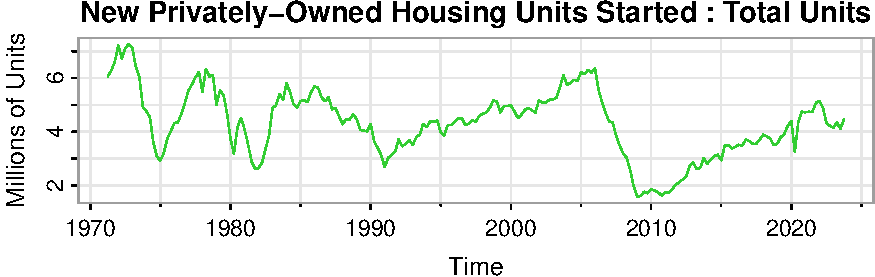
\includegraphics{STAT429Report---Copy_files/figure-latex/unnamed-chunk-4-1.pdf}

\subsection{\texorpdfstring{Homeownership Rate in the United States (RHORUSQ156N) {[}Quarterly{]} {[}Q1 '65 - Q4'23{]} \emph{Predictor variable 3}}{Homeownership Rate in the United States (RHORUSQ156N) {[}Quarterly{]} {[}Q1 '65 - Q4'23{]} Predictor variable 3}}\label{homeownership-rate-in-the-united-states-rhorusq156n-quarterly-q1-65---q423-predictor-variable-3}

The homeownership rate is the proportion of households that is owner-occupied.
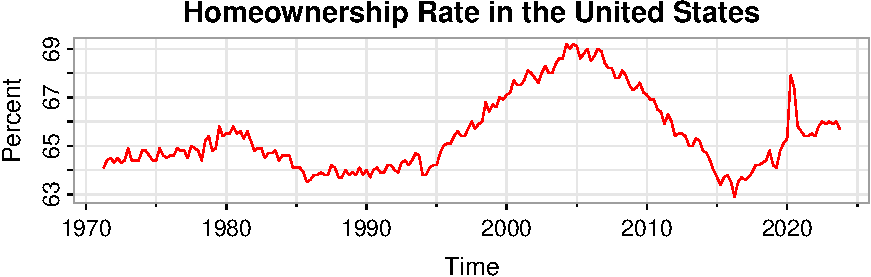
\includegraphics{STAT429Report---Copy_files/figure-latex/unnamed-chunk-5-1.pdf}

\subsection{\texorpdfstring{30-Year Fixed Rate Mortgage Average in the United States (MORTGAGE30US) {[}Weekly{]} {[}Apr'71 - Feb'24{]} \emph{Predictor variable 4}}{30-Year Fixed Rate Mortgage Average in the United States (MORTGAGE30US) {[}Weekly{]} {[}Apr'71 - Feb'24{]} Predictor variable 4}}\label{year-fixed-rate-mortgage-average-in-the-united-states-mortgage30us-weekly-apr71---feb24-predictor-variable-4}

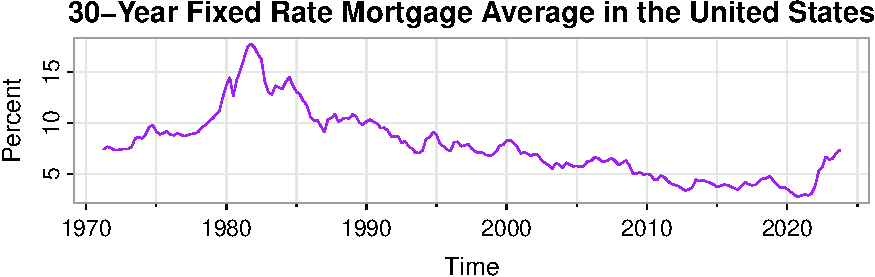
\includegraphics{STAT429Report---Copy_files/figure-latex/unnamed-chunk-6-1.pdf}

\subsection{\texorpdfstring{Consumer Price Index for All Urban Consumers: All Items Less Shelter in U.S. City Average (CUSR0000SA0L2) {[}Monthly{]} {[}Jan'47 - Jan'24{]} \emph{Additional Variable {[}NOT to be used as a predictor{]}}}{Consumer Price Index for All Urban Consumers: All Items Less Shelter in U.S. City Average (CUSR0000SA0L2) {[}Monthly{]} {[}Jan'47 - Jan'24{]} Additional Variable {[}NOT to be used as a predictor{]}}}\label{consumer-price-index-for-all-urban-consumers-all-items-less-shelter-in-u.s.-city-average-cusr0000sa0l2-monthly-jan47---jan24-additional-variable-not-to-be-used-as-a-predictor}

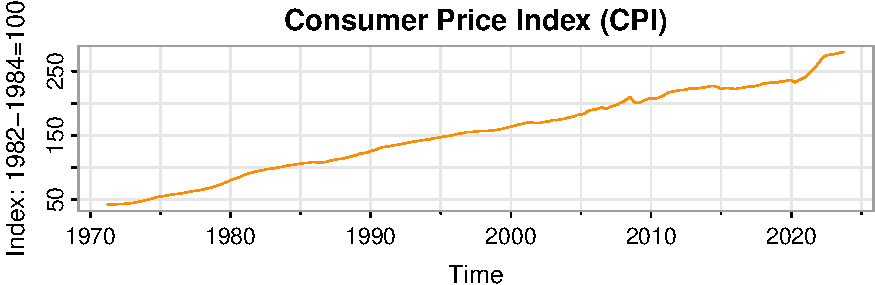
\includegraphics{STAT429Report---Copy_files/figure-latex/unnamed-chunk-7-1.pdf}

\subsection{Plans for Analysis A}\label{plans-for-analysis-a}

The time series data of median price {[}MSPUS{]} will be regressed on time \emph{(t)} and the four other independent variables. The Median Prices (outcome variable) will be pre processed by adjusting for inflation, followed by de-trending and log transformation to make it stationary and homoscedastic. The four predictor variables will be converted into quarterly series if they are not already. The Median Price will be regressed on time and other predictors to arrive at the full model. Multiple model sizes will be analyzed to find the optimum model to be selected, based on AIC/BIC criteria. Based on the p/ACF of the residuals, we may conduct regression with autocorrelated errors.

\section{Methods}\label{methods}

Preliminary adjustments indicate that median prices can be make stationary before regression with some adjustment for the heteroscastic behavior present in the series.

ADF \& KPSS tests conclude stationarity. But the series exhibits an obvious heteroscedasticity (evidenced by BP-Test), where higher levels are associated with higher variation. A BoxCox transformation is recommended.

The differenced and BoxCox transformed series passes tests of stationarity and is homoscedastic. We can now proceed with regression. We will use the step-wise algorithm to find the optimum model.

The stepwise algorithm concludes that Predictor 1 (MSACSR) and Predictor 4 (MORTGAGE30US) are significant predictors of housing prices based on AIC criteria. \emph{Check appendix for full rresults of the algorithm.} We will now carry out residual analysis:

The Ljung-Box test concludes that the residuals are not independently distributed; they exhibit serial correlation. We will carry out Regression with autocorrelated errors.

ACF cuts off after 1. PACF cuts off after 1. ARMA(1,1) looks like a good fit for the residuals. We will fit a ARMA(1,1) model and carry out forecasting.

The ACF of residuals show that they now resemble white noise. We will carry out the forecasting of the stationary series using \emph{sarima.for()} function.

\subsection{Analysis C}\label{analysis-c}

The plot of squared residuals from the ARIMA fit shows the residuals have conditional heteroscedasticity. An ARCH/GARCH model should work well to model this. We will fit three ARCH models: GARCH, IGARCH \& APARCH.

GARCH models assume stationarity. Therefore we will use the log-differenced series for GARCH model which is stationary. We need to evaluate the mean model ARMA Order and GARCH order simultaneously to fit a ARMA-GARCH model.The mean model uses ARMA that generates the forecast for the mean of the time series, while the GARCH model generates the forecast for the variance. The mean model will use an ARMA(1,1) and we will use different GARCH orders to find the best ICs to evaluate goodness of fit.

\subsection{GARCH}\label{garch}

\subsection{APARCH}\label{aparch}

\subsection{IGARCH}\label{igarch}

\section{Results}\label{results}

MSACSR (Median Sales Price of Houses Sold) and MORTGAGE30US (30 Year Fixed Rate Mortgage Average) are significant predictors of housing prices. ARIMA (1,1,1) shows the best performance among all models tested with autocorrelated errors.

We find that all three ARCH models fail to capture volatility patterns with a high degree of satisfaction. APARCH model does not seem to model negative volatility much differently from positive volatility. This may be due to very limited negative shocks experienced by the housing market, historically.We find that GARCH, APARCH \& IGARCH models predict returns differently. This results in different values of the predicted values.

\section{Discussion}\label{discussion}

A synopsis of your findings and any limitations your study may suffer from.

\newpage

\section{References}\label{references}

\phantomsection\label{refs}
\begin{CSLReferences}{0}{1}
\end{CSLReferences}

\section{Appendix (Optional)}\label{appendix-optional}

Any R codes or less important R outputs that you wanted to keep- can go in here.


\end{document}
